\chapter{Methodology and development}
\label{cha:chapter3}

\section{The Repository}

This work was done in Jupyter notebook format in a GitHub repository (\url{https://github.com/gperaza/road-network}). This repository's root contains an environment definition file and a notebooks folder. Within that folder, the repository contains one folder for the work done in Mérida, Yucatán, and other folder for the different cities in México that are beyond the scope of this report. The following notebooks are included in the Mérida folder:

\begin{enumerate}
	\item Data preparation, downloading/modeling and calculating network stats of Mérida's road network and its urban AGEBs.
	\item Analysis of the road network of Mérida and its urban AGEBs.
	\item Cluster analysis of the urban AGEBs.
\end{enumerate}

To run the code examples in this resource repository, we simply run everything in a pre-built Anaconda environment. This process is detailed in the following section.

\section{The Environment}

This project's repository contains an Anaconda environment file (i.e., .yml) for running the Jupyter notebooks on any computer. Anaconda \cite{anaconda} is a data science platform that facilitates package management and deployment. It is available for Windows, Linux and macOS. We use the Individual Edition, which is the open-source distribution of Anaconda.

First, download and install Anaconda Individual Edition. Once it is installed and running on your computer, run the following code in the terminal window:

\begin{lstlisting}[language=bash]
$ conda config --add channels conda-forge
$ conda env create --file road-network-project.yml
$ conda activate road-network-project
$ jupyter lab
\end{lstlisting}

Once you are in the active environment, open your computer's web browser and visit \url{http://localhost:8888} to access Jupyter Lab and open this work's notebook files.

\section{Data Collection}

This work uses OSMnx to download the street network of Mérida and its AGEBs, construct a graph model of it (using NetworkX), correct, analyze, and visualize at municipal, and neighborhood (AGEB) scales. 

In order to get the street network of Mérida, we define a function to download and save the graph of the municipality, or, if already present, load it as an NetworkX graph object:

\begin{lstlisting}[language=Python]
def get_roads_osmnx(places, update=False, proj=False, crs=None):

	dirpath = pathlib.Path('./data/networks/')
	filepath = dirpath/'merida-road.graphml'
	logpath = dirpath/'log'

	if filepath.exists() and not update:
		G = ox.load_graphml(filepath)
	else:
		# get drivable public streets network, aka road network, without service roads,
		# e.g. private, parking lots, etc.
		# use retain_all if you want to keep all disconnected subgraphs (e.g. when your places aren't adjacent)
		G = ox.graph_from_place(places, network_type='drive')
		ox.save_graphml(G, filepath=filepath, gephi=False)
	
	if proj:
		G = ox.project_graph(G, to_crs=crs)
	
	print(f"Graph created at: {G.graph['created_date']}")
	return G, *ox.graph_to_gdfs(G)
	
places = [{'county' : 'Merida', 'state' : 'Yucatan', 'country' : 'Mexico'}]
G_proj, nodes_proj, edges_proj = get_roads_osmnx(places, update=False, proj=True, crs=3857)
\end{lstlisting}

OSMnx geocodes the query "Merida, Yucatan, Mexico" to retrieve the place boundaries of that city from the Nominatim API, retrieves the drivable street network data within those boundaries from the Overpass API, constructs a graph model (via NetworkX), then simplifies/corrects its topology such that nodes represent intersections and dead-ends, and edges represent the street segments linking them. It also saves the constructed graph as a GraphML file to not re-download the same data again.

OSMnx models all networks as NetworkX MultiDiGraph objects. You can convert to:

\begin{itemize}
	\item Undirected MultiGraphs.
	\item DiGraphs without (possible) parallel edges.
	\item GeoPandas node/edge GeoDataFrames.
\end{itemize}

In the function, we also convert the graph to node and edge GeoDataFrames. Additionally, we project the graph to the WGS84 Pseudo-Mercator  CRS.

Remember that one of the most commonly used CRS is the WGS84 latitude-longitude projection. This can be referred to using the authority code "EPSG:4326". However, such EPSG is in degree units. For that reason, we will use an alternative option which is the "EPSG:3857" that is measured in meters. This projected coordinate system is the one that Google, OpenStreetMap, Bing, ArcGIS, ESRI, etc. use for rendering their maps \cite{epsg3857}.

In the case of the Mérida's urban AGEBs, we collect geographic data from the Institute of Statistics and Geography's (INEGI) National Geoestatistical Framework (MG) and socio-demographic data from INEGI's 2020 Population and Housing Census (2020 Census) conducted from March 2 to March 27, 2020 \cite{2020census}.

The MG is a mexican unique national system designed by INEGI to correctly reference statistical information from censuses and surveys with the corresponding geographic locations \cite{manualMGN}. It is conformed by geostatistical areas divided into three dissaggregation areas (see Figure \ref{fig:MGN_divisions}):

\begin{itemize}
	\item State geoestatistical areas (AGEE).
	\item Municipal geoestatistical areas (AGEM).
	\item Basic geoestatistical areas (AGEB).
	\begin{itemize}
		\item Rural AGEB.
		\item Urban AGEB.
	\end{itemize}
\end{itemize}

\begin{figure}[h!]
	\centering
	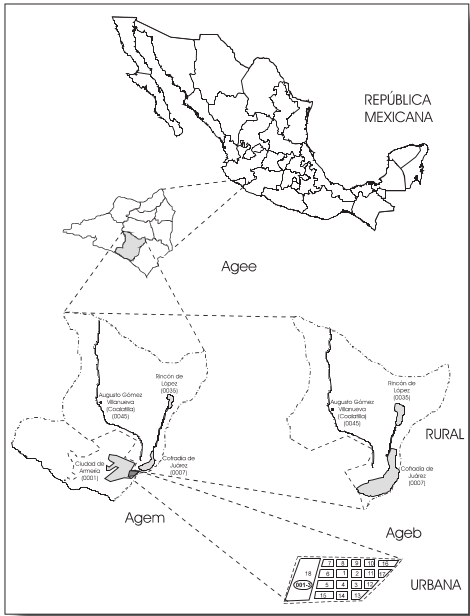
\includegraphics[width=0.6\textwidth]{Figures/MGN_divisions.png}
	\caption{MG dissaggregation areas. Retrieved from: \cite{manualMGN}.
		\label{fig:MGN_divisions}}
\end{figure}

Urban AGEBs are the geographic area, subdivision of municipal areas, occupied by a set of blocks, generally ranging from 1 to 50, perfectly delimited by streets, avenues, walkways or any other easily identifiable feature on the ground and whose land use is mainly residential, industrial, services, commercial, etc., only assigned within urban localities (see Figure \ref{fig:ageb_division}).

\begin{figure}[h!]
	\centering
	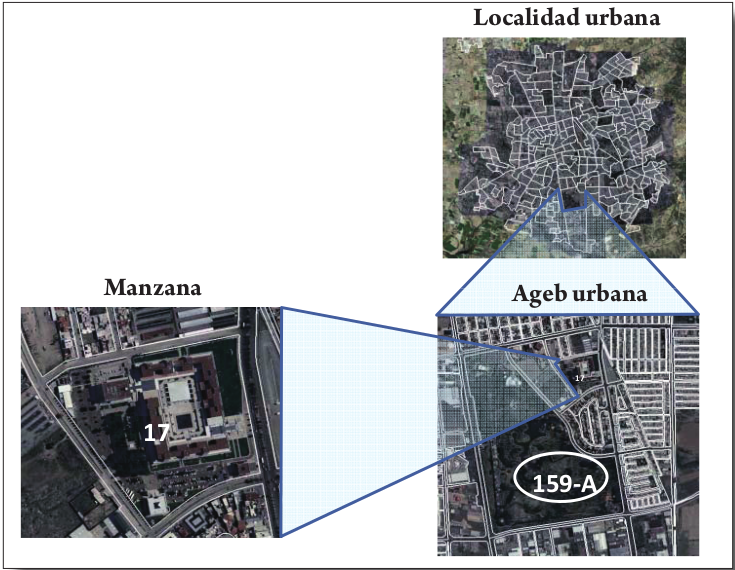
\includegraphics[width=0.7\textwidth]{Figures/ageb_division.png}
	\caption{Urban AGEB dissaggregation areas. Retrieved from: \cite{manualMGN}.
		\label{fig:ageb_division}}
\end{figure}

We download the MG data from \cite{MG_data}, which contains the shapefiles of every dissaggregation area of every mexican state. It is made up of 32 folders, each one named by the geoestatistical key of the federal entity (from 1 to 32), with a national total of 2,469 municipal geoestatistical areas, 45,397 polygons of rural localities, and 4,911 polygons of urban localities, 295,779 points of rural localities, 350 polygons of island territory, 17,469 basic rural geostatistical areas, 63,982 basic urban geostatistical areas and 2,513,853 urban and rural blocks (including scattered hamlets); the information maintains associated names and geostatistical keys as attributes.

The MG references every dissaggregation area with a unique numeric key. The structure of such geostatistical key is represented in Figure \ref{fig:key_structure}.

\begin{figure}[h!]
	\centering
	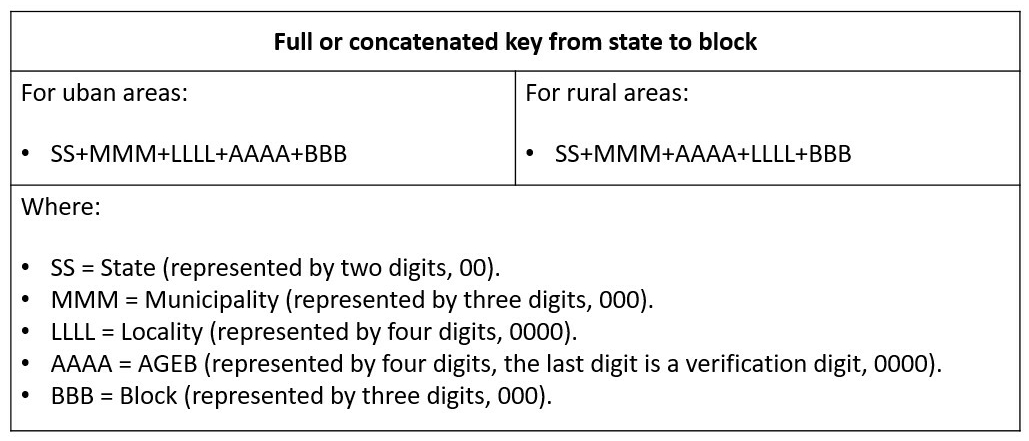
\includegraphics[width=0.8\textwidth]{Figures/key_structure.jpg}
	\caption{MG's geostatistical key structure. Retrieved from: \cite{manualMGN}.
		\label{fig:key_structure}}
\end{figure}


Every state folder of the MG is composed of three subfolders:

\begin{itemize}
	\item Catalogs (catálogos): contains the product catalogs and documentation.
	\item Data set (conjunto\_de\_datos): contains 32 folders, each one corresponding to the state geoestatistical key.
	\item Metadata (metadatos): contains 32 files, each one with the corresponding state geostatistical key, in xml and txt format, and a generic metadata with national information.
\end{itemize}

The file names are formed with the state geoestatistical key and the following suffixes of the file content: 

Where \textbf{ee} corresponds to the state geoestatistical key (from 01 to 32).

\begin{table*}[h!]
	\centering
	\label{tab:MG_filenames}
	\footnotesize
	\begin{tabular}{ l l }
		ee\textbf{ent} & State geoestatistical areas \\
		ee\textbf{mun} & Municipal geoestatistical areas \\
		ee\textbf{ar} & Basic rural geoestatistical areas \\
		ee\textbf{l} & Polygon of urban and rural localities \\
		ee\textbf{lpr} & Rural point locations \\
		ee\textbf{ti} & Island territory\\
		ee\textbf{a} & Basic urban geoestatistical areas \\
		ee\textbf{m} & Block polygons\\
		ee\textbf{fm} & Block fronts \\
		ee\textbf{e} & Road axes \\
		ee\textbf{cd} & Scattered hamlet \\
		ee\textbf{sia} & Complementary area-type services and information (green areas, medians, traffic circles) \\
		ee\textbf{sil} & Complementary line-type services and information
		(rivers, railroads, streams) \\
		ee\textbf{sip} & Complementary point-type services and information
		(municipal palaces, parks or gardens, etc.) \\
		ee\textbf{pe} & External polygon \\
		ee\textbf{pem} & External polygon of blocks \\
	\end{tabular}
\end{table*}

Layers with suffix \textbf{ti}, \textbf{cd}, \textbf{pe}, \textbf{pem}, \textbf{sia}, \textbf{sil}, \textbf{sip}, are included only if the locality has this type of information.

INEGI's 2020 census data was downloaded from \cite{2020census} on the main results by AGEB and urban block subsection. In this subsection we can download data from every mexican state in a CSV (comma-separated values) file.

In this work, we are only using the MG Yucatán folder (31\_yucatan) and the file of the basic urban geoestatistical areas (31a.shp), as well as census data from Yucatán.


\section{Data Exploration and Preparation}


\section{Data Modeling}


